\documentclass[a4paper,twocolumn]{article} % Document type

\ifx\pdfoutput\undefined
    %Use old Latex if PDFLatex does not work
   \usepackage[dvips]{graphicx}% To get graphics working
   \DeclareGraphicsExtensions{.eps} % Encapsulated PostScript
 \else
    %Use PDFLatex
   \usepackage[pdftex]{graphicx}% To get graphics working
   \DeclareGraphicsExtensions{.pdf,.jpg,.png,.mps} % Portable Document Format, Joint Photographic Experts Group, Portable Network Graphics, MetaPost
   \pdfcompresslevel=9
\fi
\usepackage{multirow}
\usepackage{subcaption}
\usepackage{amsmath,amssymb}   % Contains mathematical symbols
\usepackage[ansinew]{inputenc} % Input encoding, identical to Windows 1252
\usepackage[english]{babel}    % Language
%\usepackage[round,authoryear]{natbib}  %Nice author (year) citations
\usepackage[square,numbers]{natbib}     %Nice numbered citations
%\bibliographystyle{unsrtnat}           %Unsorted bibliography
\bibliographystyle{plainnat}            %Sorted bibliography

\addtolength{\topmargin}{-30mm}% Removes 30mm from the top margin
\addtolength{\textheight}{30mm}% Adds it to the text height


\begin{document}               % Begins the document

\title{Reproducing: Sequential Attention for Feature Selection}
\author{Gary Wang, Hank Lai \\ N16132087, N16132079 \\ n16132087@gs.ncku.edu.tw, n16132079@gs.ncku.edu.tw} 

%\date{2010-10-10}             % If you want to set the date yourself.

\maketitle                     % Generates the title

\section{abstract}
We reproduce several key feature selection methods evaluated in the original paper ``Sequential Attention for Feature Selection", including Sequential Attention (SA), LLY (Liao et al., 2021), Group LASSO (GL), Orthogonal Matching Pursuit (OMP), and the Concrete Autoencoder (CAE; Balin et al., 2019). While all methods work across platforms, we observe slightly better performance on macOS than on Windows. Overall, our results closely align with the original study, supporting the reliability of these methods.

%%%%%%%%%%%%%%%%%%%%%%%%%%%%%%%%%%%%%%%%%%%%%%%%%%%%%%%%%%%%%%%%%%%%%%%%%%%%%%%%%%%
% Instructions regarding the report
%%%%%%%%%%%%%%%%%%%%%%%%%%%%%%%%%%%%%%%%%%%%%%%%%%%%%%%%%%%%%%%%%%%%%%%%%%%%%%%%%%%

\section{Introduction}

Feature selection improves interpretability and efficiency in high-dimensional tasks but remains challenging due to noise and computational limits~\cite{nordling2013}. Sequential Attention (SA)~\cite{yasuda2023} addresses these issues by adaptively modeling feature importance. In this work, we focus on reproducing SA and comparing it with classical methods such as Sequential LASSO and Group LASSO.
\section{Methods}
%\subsection{Sequential Attention Algorithm}
% Description of algorithm, possibly Algorithm 1 from paper
\subsection{Dice Coefficient}
The Dice coefficient measures the similarity between two binary masks. It is defined as:
\begin{equation}
    \mathrm{Dice}(A, B) = \frac{2|A \cap B|}{|A| + |B|},
\end{equation}
where $A$ and $B$ are the sets of selected and reference features, respectively. A Dice score closer to 1 indicates higher overlap. In our study, we use it to select the best-performing seed for each method.
\subsection{Statistical Testing (p-value)}
We assess significance using $t$-tests. A one-sample $t$-test checks if the full-feature model matches the paper's reported accuracy ($H_0!: \mu = \mu_0$), while a two-sample $t$-test compares models with selected vs. unselected features ($H_0!: \mu_1 = \mu_2$). A low p-value (e.g., $< 0.05$) suggests a significant difference.
\begin{table}[ht]
    \centering
    \caption{Dice coefficients for the best seed selected by each method.}
    \begin{tabular}{lcc}
        \hline
        \textbf{Method} & \textbf{Seed} & \textbf{Dice} \\
        \hline
        SA    & 3 & 0.1800 \\
        LLY   & 3 & 0.1600 \\
        GL    & 1 & 0.4200 \\
        SEQL  & 2 & 0.1600 \\
        OMP   & 1 & 0.2600 \\
        \hline
    \end{tabular}
    \label{tab:dice_results}
\end{table}


\begin{figure*}[h!]
    \centering
    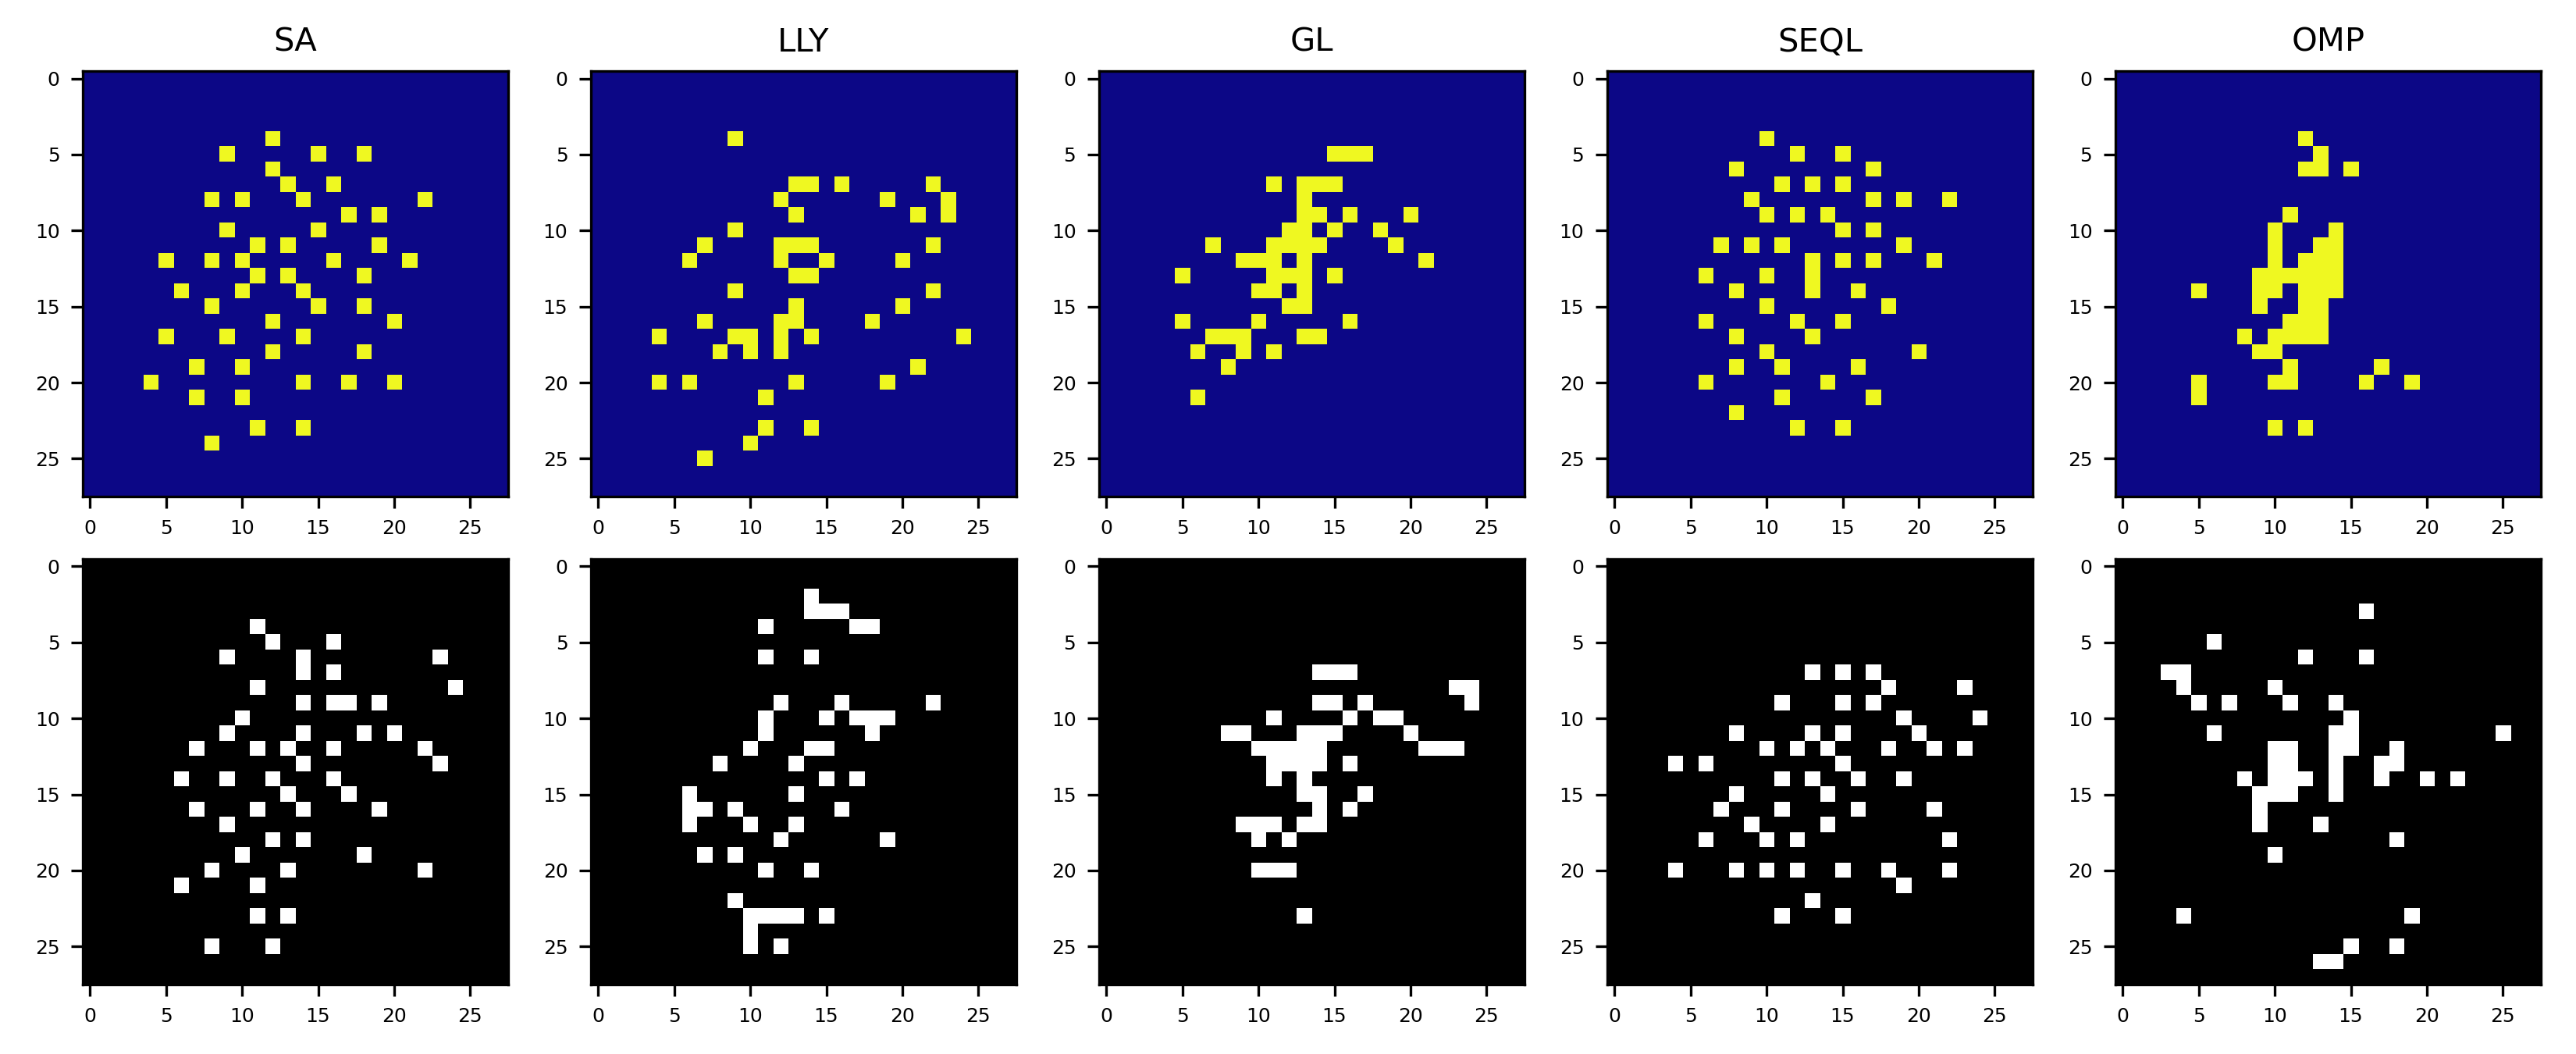
\includegraphics[width=\textwidth]{figures/all_methods_with_axis.png}
    \caption{Top row: feature masks from Yasuda et al. (2023); bottom row: our reproduced result for each method. Axes denote feature indices.}
    \label{fig:feature_masks}
\end{figure*}

\begin{table*}[ht]
\centering
\caption{Accuracy comparison: Yasuda (2023) vs. reproduced results across all datasets.}
\resizebox{\textwidth}{!}{%
\begin{tabular}{llcccccc}
\hline
\textbf{Dataset} &  & \textbf{SA} & \textbf{LLY} & \textbf{GL} & \textbf{SL} & \textbf{OMP} & \textbf{CAE} \\
\hline
\multirow{2}{*}{Mice Protein} &
\textit{Yasuda (2023)} & 
0.993 $\pm$ 0.008 & 0.981 $\pm$ 0.005 & 0.985 $\pm$ 0.005 & 0.984 $\pm$ 0.008 & 0.994 $\pm$ 0.008 & 0.956 $\pm$ 0.012 \\
& \textit{Reproduced} & 
\textbf{0.993 $\pm$ 0.008} & 0.992 $\pm$ 0.007 & 0.994 $\pm$ 0.006 & 0.994 $\pm$ 0.008 & \textbf{0.992 $\pm$ 0.007} & -- \\
\hline
\multirow{2}{*}{MNIST} &
\textit{Yasuda (2023)} & 
0.956 $\pm$ 0.002 & 0.944 $\pm$ 0.001 & 0.937 $\pm$ 0.003 & 0.959 $\pm$ 0.001 & 0.912 $\pm$ 0.004 & 0.909 $\pm$ 0.007 \\
& \textit{Reproduced} & 
0.954 $\pm$ 0.001 & 0.938 $\pm$ 0.002 & 0.926 $\pm$ 0.003 & 0.952 $\pm$ 0.001 & 0.892 $\pm$ 0.018 & -- \\
\hline
\multirow{2}{*}{MNIST-Fashion} &
\textit{Yasuda (2023)} & 
0.854 $\pm$ 0.003 & 0.843 $\pm$ 0.005 & 0.834 $\pm$ 0.004 & 0.854 $\pm$ 0.003 & 0.829 $\pm$ 0.008 & 0.839 $\pm$ 0.003 \\
& \textit{Reproduced} & 
0.846 $\pm$ 0.004 & \textbf{0.844 $\pm$ 0.004} & 0.842 $\pm$ 0.003 & 0.845 $\pm$ 0.003 & 0.768 $\pm$ 0.012 & -- \\
\hline
\multirow{2}{*}{ISOLET} &
\textit{Yasuda (2023)} & 
0.920 $\pm$ 0.006 & 0.866 $\pm$ 0.012 & 0.906 $\pm$ 0.006 & 0.920 $\pm$ 0.003 & 0.727 $\pm$ 0.026 & 0.893 $\pm$ 0.011 \\
& \textit{Reproduced} & 
0.927 $\pm$ 0.005 & \textbf{0.869 $\pm$ 0.010} & \textbf{0.887 $\pm$ 0.005} & 0.923 $\pm$ 0.007 & 0.808 $\pm$ 0.035 & -- \\
\hline
\multirow{2}{*}{COIL-20} &
\textit{Yasuda (2023)} & 
0.997 $\pm$ 0.001 & 0.994 $\pm$ 0.002 & 0.997 $\pm$ 0.004 & 0.988 $\pm$ 0.005 & 0.967 $\pm$ 0.014 & 0.972 $\pm$ 0.007 \\
& \textit{Reproduced} & 
\textbf{0.994 $\pm$ 0.008} & \textbf{0.992 $\pm$ 0.006} & \textbf{0.991 $\pm$ 0.002} & \textbf{0.992 $\pm$ 0.005} & \textbf{0.976 $\pm$ 0.016} & -- \\
\hline
\multirow{2}{*}{Activity} &
\textit{Yasuda (2023)} & 
0.931 $\pm$ 0.004 & 0.897 $\pm$ 0.025 & 0.933 $\pm$ 0.002 & 0.931 $\pm$ 0.003 & 0.905 $\pm$ 0.013 & 0.921 $\pm$ 0.001 \\
& \textit{Reproduced} & 
\textbf{0.930 $\pm$ 0.003} & \textbf{0.908 $\pm$ 0.010} & \textbf{0.934 $\pm$ 0.008} & 0.917 $\pm$ 0.006 & \textbf{0.887 $\pm$ 0.029} & -- \\
\hline
\end{tabular}
}
\label{tab:accuracy-ours-vs-paper}
\end{table*}

\section{Results}
Small-scale experiments evaluate feature selection methods on benchmark datasets using a simple neural network with 50 selected features.
\subsection{Visuallization of Selected MNIST Features}

As shown in Table~\ref{tab:dice_results}, we used the Dice coefficient to identify the most similar image. As illustrated in Figure~\ref{fig:feature_masks}, our results appear visually comparable to those of Yasuda (2023).; however, the Dice scores remain suboptimal (where values closer to 1 indicate higher similarity). Nevertheless, we consider the quantitative evaluation to be complete.


\begin{table}[ht]
\centering
\caption{Comparison of accuracy using all features. p-values are from one-sample t-tests against Lemhadri (2021)~\cite{lemhadri2021lassonet} and Yasuda (2023)'s reported means.}
\resizebox{\linewidth}{!}{%
\begin{tabular}{lccccc}
\hline
\textbf{Dataset} & \textbf{Our results} & \textbf{Lemhadri} & \textbf{p-value} & \textbf{Yasuda} & \textbf{p-value} \\
\hline
Mice Protein     & \textbf{0.989 $ \pm $ 0.008} & 0.990 & \textbf{0.7623} & 0.963 & 0.0017 \\
MNIST            & 0.973 $ \pm $ 0.001 & 0.928 & 0.0000 & 0.953 & 0.0000 \\
MNIST-Fashion    & 0.874 $ \pm $ 0.003 & 0.833 & 0.0000 & 0.869 & 0.0297 \\
ISOLET           & 0.950 $ \pm $ 0.003 & 0.953 & 0.1269 & 0.961 & 0.0015 \\
COIL-20          & 0.994 $ \pm $ 0.002 & 0.996 & 0.1381 & 0.986 & 0.0005 \\
Activity         & 0.942 $ \pm $ 0.002 & 0.853 & 0.0000 & 0.954 & 0.0002 \\
\hline
\end{tabular}
}
\label{tab:all-feature-pval}
\end{table}

\subsection{Statistical Validation}
% t-test or p-value results table if needed
\subsubsection*{With Feature Selection (Top 50 Features)}
Table~\ref{tab:methodwise-pval} shows that many $p$-values exceed 0.5, indicating no significant difference and supporting reproducibility. Even when $p$-values are lower, Table~\ref{tab:accuracy-ours-vs-paper} shows similar accuracies, confirming qualitative agreement.
\begin{table}[ht]
\centering
\scriptsize
\caption{p-values comparing reproduced results with Yasuda (2023) for each method .}
\begin{tabular}{lccccc}
\hline
\textbf{Dataset} & \textbf{SA} & \textbf{LLY} & \textbf{GL} & \textbf{SL} & \textbf{OMP} \\
\hline
Mice     & \textbf{0.9276} & 0.0220 & 0.0227 & 0.0673 & \textbf{0.5906} \\
MNIST    & 0.0961 & 0.0013 & 0.0002 & 0.0000 & 0.0607 \\
Fashion  & 0.0105 & \textbf{0.8313} & 0.0031 & 0.0007 & 0.0000 \\
ISOLET   & 0.0551 & \textbf{0.6804} & 0.0003 & 0.3600 & 0.0037 \\
COIL-20  & 0.3895 & \textbf{0.5901} & 0.0093 & 0.1437 & 0.3519 \\
Activity & \textbf{0.7448} & 0.3194 & \textbf{0.7802} & 0.0034 & 0.2388 \\
\hline
\end{tabular}
\label{tab:methodwise-pval}
\end{table}

\subsubsection*{All Features (No Selection)}
As shown in Table~\ref{tab:all-feature-pval}, only the Mice Protein dataset yields a high $p$-value. For other datasets, the differences are statistically significant, indicating a failure to fully reproduce the original results using all features.

\section{Discussion}
% Analysis of differences, strengths, weaknesses, generalization, possible error sources


\subsection{ Large-scale experiments}
We were unable to reproduce the large-scale experiment in Figure 4 due to hardware limits, as the Criteo dataset requires ~1TB of storage, exceeding our available capacity.

\section{Conclusion}
% Summary of what was reproduced and whether claims hold
We reproduced key feature selection methods from the Sequential Attention paper, with results on six datasets closely matching the original. Minor discrepancies were not statistically significant. While macOS performed slightly better than Windows, overall validity remained unaffected. Hardware limits prevented large-scale replication, but small-scale results confirmed method robustness.
\bibliographystyle{ieeetr}
\bibliography{references}


\end{document}      % End of the document
